%================================================================
\section{Background}\label{sec:Theory}
%================================================================

\subsubsection*{New outline}

\begin{itemize}
    \item Just focus on dim reduction (no parameter estimation)
    \item Experiments
    \begin{itemize}
        \item Conv-VAE MNIST (f.ex. 0-4) *
        \item $\beta$-VAE MNIST *
        \item InfoVAE MNIST *
        \item InfoVAE HH *
        \item Maybe: InfoVAE OU *
        \item LSTM or Transformer VAE HH (deterministic)
        \item Maybe: try models on Ornstein–Uhlenbeck (OU) process (stochastic) \url{https://stat.pitt.edu/si/ou.pdf}
    \end{itemize}
    \item Model goodness qualitatively by comparing simulation vs generative model
    \item use t-SNE for visualizing latent space
    \item Quantitative:
    \begin{itemize}
        \item Reconstruction error over latent dimensionality
    \end{itemize}
\end{itemize}

\subsubsection*{Old outline}

\begin{itemize}
    \item Autoencoders (brief)
    \begin{itemize}
        \item Purpose
        \item Architecture
        \item Optimization (reconstruction loss)
    \end{itemize}
    \item Variational autoencoders
    \begin{itemize}
        \item Key difference between AE and VAE
        \item VAE optimization (reconstruction loss + regularization)
        \item Reparametrization trick
    \end{itemize}
    \item $\beta$-VAE
    \item Convolutional VAE (maybe Method)
    \begin{itemize}
        \item Traditional CNN
        \item If time, modern CNN with Fourier transforms
    \end{itemize}
    \item LSTM-based VAE (maybe Method)
    \begin{itemize}
        \item RNN background
        \item LSTM
    \end{itemize}
    \item Latent perturbation / interpreting latent features 
\end{itemize}

%----------------------------------------------------------------
\subsection{Autoencoders}
%----------------------------------------------------------------
Autoencoders are a method of dimensionality reduction, used for data compression or for extracting the most important features of a dataset. Some input, such as an image, is send into a first part, the \textbf{encoder}, see \autoref{fig:ae} where it is shrunk to the lowest possible \textbf{latent feature} representation. What is meant by the lowest possible feature representation is one in which a replication of the input (up to a given “quality”) can be reproduced by (typically) reversing the encoder in what is called a \textbf{decoder}. The goal of the (auto)encoder is typically to create the latent feature representation, while the decoder is there to reconstruct the input from this reduced representation so that we can find the error of the reconstruction compared to the input. The choice of encoder is up to the user and is typically chosen depending on the type of input; convolutional networks for images, recurrent neural networks for sequential data such as time-series data, and so on.

\begin{figure}[!htb]
 \centering
 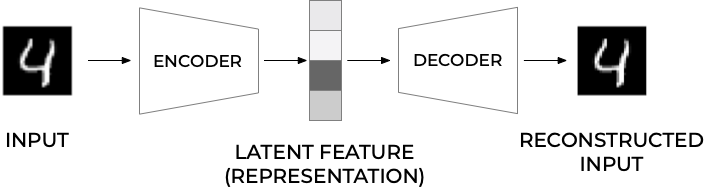
\includegraphics[scale=0.5]{ae1.png}
 % ae1.png: 711x193 px, 72dpi, 25.08x6.81 cm, bb=0 0 711 193
 \caption{\textbf{Autoencoder representation}: Here, an image depicting the digit 4 from the MNIST dataset is first sent through an encoder which compresses the image to a lower-dimensional (latent feature) representation. Then, the compressed representation is sent through a decoder which tries to reconstruct the original image.}
 \label{fig:ae}
\end{figure}

Although autoencoders can compress and recreate data easily, there is no stochasticity involved, so they are not suited to create new data fitting a specific class. As an example, an autoencoder trained on pictures of chairs may recreate the specific chairs it was trained on, but it will not be able to span the entire space of 'chairness`` and produce a series of new and original images of chairs. Another issue is that the latent space of regular autoencoders may not be continuous, making generation and interpretation of specific features difficult or impossible.
In order to introduce stochasticity (as well as continuous and more 'useful' latent spaces) into the equation we go to \textbf{Variational Auto Encoders (VAEs)}

\subsection{Variational Autoencoders (VAEs)}
In a very simplified way, one can say that stochasticity in VAEs is introduced in the data stored in the latent feature space (see \autoref{fig:ae}), where instead of storing a single output value per feature in the layer, a probability distribution is stored (a mean and an std for each feature). This ensures that specific features are continuous around their mean (via their std), and that they can be separated enough to be distinguishable (via their mean).

This probability distribution in the feature layer allows us to pick samples and create new output that is (hopefully) still recognizable as what the VAE is intended to generate, while still completely new and not seen in the training data. 

%If we label these samples \textbf{h} (latent variables), and our output \textbf{x},
To obtain a good generative model, one needs to maximize the marginal likelihood $p(x)$ over all x. This is not always an easy expression to handle, as one either must know the true distribution of the data, or do an infeasible integral over latent parameters. The workaround for this issue is to derive an expression for what is known as ELBO, or Evidence Lower Boundary (\autoref{eqn:elbo}). Evidence means just the loglikelihood of the observed data (input).
Given a parametrized encoder whose goal is to be as close as possible to the ground truth distributions; $q_\phi(z|x)\approx p(z|x)$ the ELBO can be written as:

\begin{equation}\label{eqn:elbo}
 \mathbb{E}_{q_\phi(z|x)}\left[\log \frac{p(x,z)}{q_\phi(z|x)}  \right]
\end{equation}

As the name tells us, this is the lower boundary, so in other words we wish to maximize this expression to optimize our model. By using the chain rule of probability on the expression for ELBO we can rewrite it as

\begin{equation}\label{eqn:loss}
 \mathbb{E}_{q_\phi(z|x)}\left[\log \frac{p(x,z)}{q_\phi(z|x)}  \right]
 = \mathbb{E}_{q_\phi(z|x)}[\log p_\theta (x|z)] -D_{KL}(q_\phi(z|x)||p(z))
\end{equation}

Note that we now have a new parameter function $p_\theta(x|z)$, which takes samples from the latent space z and creates new output z. The $\theta$ indicates that this is also parametrized. All the stochasticity we required is already included in creating the latent space, so this function is deterministic. The same sample from z will create the same output. The second term is known as the Kullback-Liebler divergence, which is a measure of how much two probability distributions differ.

Another thing to note in \autoref{eqn:loss} is that we now have a function $q_\phi(z|x)$ that functions as an encoder, taking data from x into z, and a function $p_\theta(x|z)$ that functions as a decoder, taking a sample z and turning it into output x.
The first term on the right hand side in \autoref{eqn:loss} can be interpreted as the reconstruction error, making sure our model produces latent features that can be used to recreate input data. The second term measures how similar our encoder is to a prior $p(z)$, and is often called a regularization term. \\ 

\subsubsection{$\beta$-VAE}
There are still a couple of issues to contend with for us. One is that features in the latent space can become entangled; which in a VAE working on creating faces the feature controlling the angle of the head could be tangled up with the one determining how much a person smiled. So, if you generated a person looking to the left, he would always be sad, but one looking to the right would always be happy. This problem is solved elegantly by introducing a hyperparameter $\beta >1$ in front of the KL-divergence term in the ELBO equation:

\begin{equation}\label{eqn:beta}
 \mathbb{E}_{q_\phi(z|x)}\left[\log \frac{p(x,z)}{q_\phi(z|x)}  \right]
 = \mathbb{E}_{q_\phi(z|x)}[\log p_\theta (x|z)] -\beta D_{KL}(q_\phi(z|x)||p(z))
\end{equation}

This parameter forces your model optimization to consider the chosen prior. Say you chose something sensible, like a multivariate Gaussian, the model will now force your encoded values closer to such a distribution. The beta will increase the cost of adding features to your latent layer, reducing degeneration (a model for drawing faces could have a feature for hair color, one for eye color, as well as one encoding both at the same time. This last one is entirely superfluous, and $\beta$-VAE should help eliminate such errant features).

\subsubsection{InfoVAE}
%Another potential issue with VAEs is that our decoder may simply recreate good results without using the samples taken from the latent space at all, or our latent space.

%encoder maps q(z|x) from X to z, decoder P(x|z) to predict specific x from z.
%draw datapoint  x_i:p(x|z), draw latent z_i: p(z)
%prob of x generated by z

Another potential issue with VAEs is that our encoder can produce the same latent features for any input x, so when our decoder samples from this it in effect samples from the distribution of input data, not from any learned and significant features.
This might not be such a big issue if you only wish to create a VAE that generates images, but if you wish to use your encoder to learn specific information, such as ''which measurable quantities are important to create this specific experimental data``, you need to make sure the latent space containts useful features.
%This issue will tend to occur if the regularization term is too strong, or too weak..
InfoVAE tackles both this problem as well as the one $\beta$-VAE handled (in fact it can be shown that $\beta$-VAE is a special case of InfoVAE).
To set up the training objective of InfoVAE it is best to start from an alternate, but equivalent up to a constant, formulation of \autoref{eqn:loss} (Zhao et al. 2019, AAAI-19);

\begin{equation} \label{eqn:4}
 \mathbb{E}_{q_\phi(z|x)}\left[\log \frac{p(x,z)}{q_\phi(z|x)}  \right]
 =-D_{KL}(q_\phi(z)||p(z))-\mathbb{E}_{q_\phi(z)}[D_{KL}(q_\phi(x|z)||p_\theta(x|z))].
\end{equation}

A further issue found in VAEs arises from the fact that the dimensions of inputs x is typically much larger than the feature space z. This is known as Modeling Bias, and applies to both divergences in  \autoref{eqn:4}. If these two divergences are inversely increasing, the error from the last term on the RHS of \autoref{eqn:4} will dwarf the other one and the divergences of the latent space will become insignificant.

To handle all the aforementioned issues with the standard VAE we modify the training objective in some specific ways. In order to emphasize the importance of divergence in the latent space we multiply the first term on the RHS of \autoref{eqn:4} by a scaling hyperparameter $\lambda$. We then add a new term to handle the tendency of not using the sample z from latent space when decoding. This term is based on the mutual information between z and x, $I_{q_\phi}(x,z)$. Note that this term is positive, so we wish to minimize the mutual information. Our new objective is then

\begin{align}
 \mathbb{E}_{q_\phi(z|x)}\left[\log \frac{p(x,z)}{q_\phi(z|x)}  \right]_{InfoVAE}
 =&-\lambda D_{KL}(q_\phi(z)||p(z))\\ \nonumber
 &-\mathbb{E}_{q_\phi(z)}[D_{KL}(q_\phi(x|z)||p_\theta(x|z))]\\ \nonumber
 &+\alpha I_{q_\phi(x,z)}(x;z).
 \label{eqn:4}
\end{align}

This expression is not readily optimizable, but the further derivations are not very illuminating.\\
This equation returns to the standard ELBO by setting the new hyperparameters to $\alpha=0$ and $\lambda=1$, while a $\lambda > 0$ and $\alpha+\lambda-1=0$ returns us to $\beta$-VAE.


\subsubsection{the mathemathics of autoencoders}
This gets close to MHJ lecture notes, do we need it?\\
If we define the input as \textbf{x}, the encoder can be seen as a function working on it via some weights to be determined, \textbf{W}; \\$\textbf{h}=f(\mathbf{x},\mathbf{W})$.\\
The decoder is then a function working with \textbf{h} as input, and a new set of weights \textbf{V}, creating the reconstructed output $\tilde{x}$; \\$\tilde{x}=g(\mathbf{h},\mathbf{V})$.\\
Now we have an $x$ and an $\tilde{x}$ we can compare to find a reconstruction error and evaluate our feature layer.


\subsection{RNN}
Recurrent Neural Networks, or RNNs, are a type of neural network designed/structured to handle sequential, often time dependent, data. Where a typical Feed Forward Neural Network sends a single input vector \textbf{x} through an arbitrary number of hidden layers \textbf{h} to reach an output \textbf{y}, a recurrent network will send a separate input \textbf{x$<$t$>$} into a separate hidden layer \textbf{h$<$t$>$} for  every step of the sequence (or every time step), see \autoref{fig:RNN}. Each of these hidden layers will also receive input from the previous sequential hidden layer in order to incorporate the sequential nature of the input data. For each set of input data \textbf{x$<$t$>$} we will receive a separate output data \textbf{y$<$t$>$}, which in turn can be used to compute a loss for each sequential step. One will then require a total loss function over all steps, which can simply be the sum over all sequential steps. This loss is then backpropagated through the whole network. 

\begin{figure}[!htb]
 \centering
 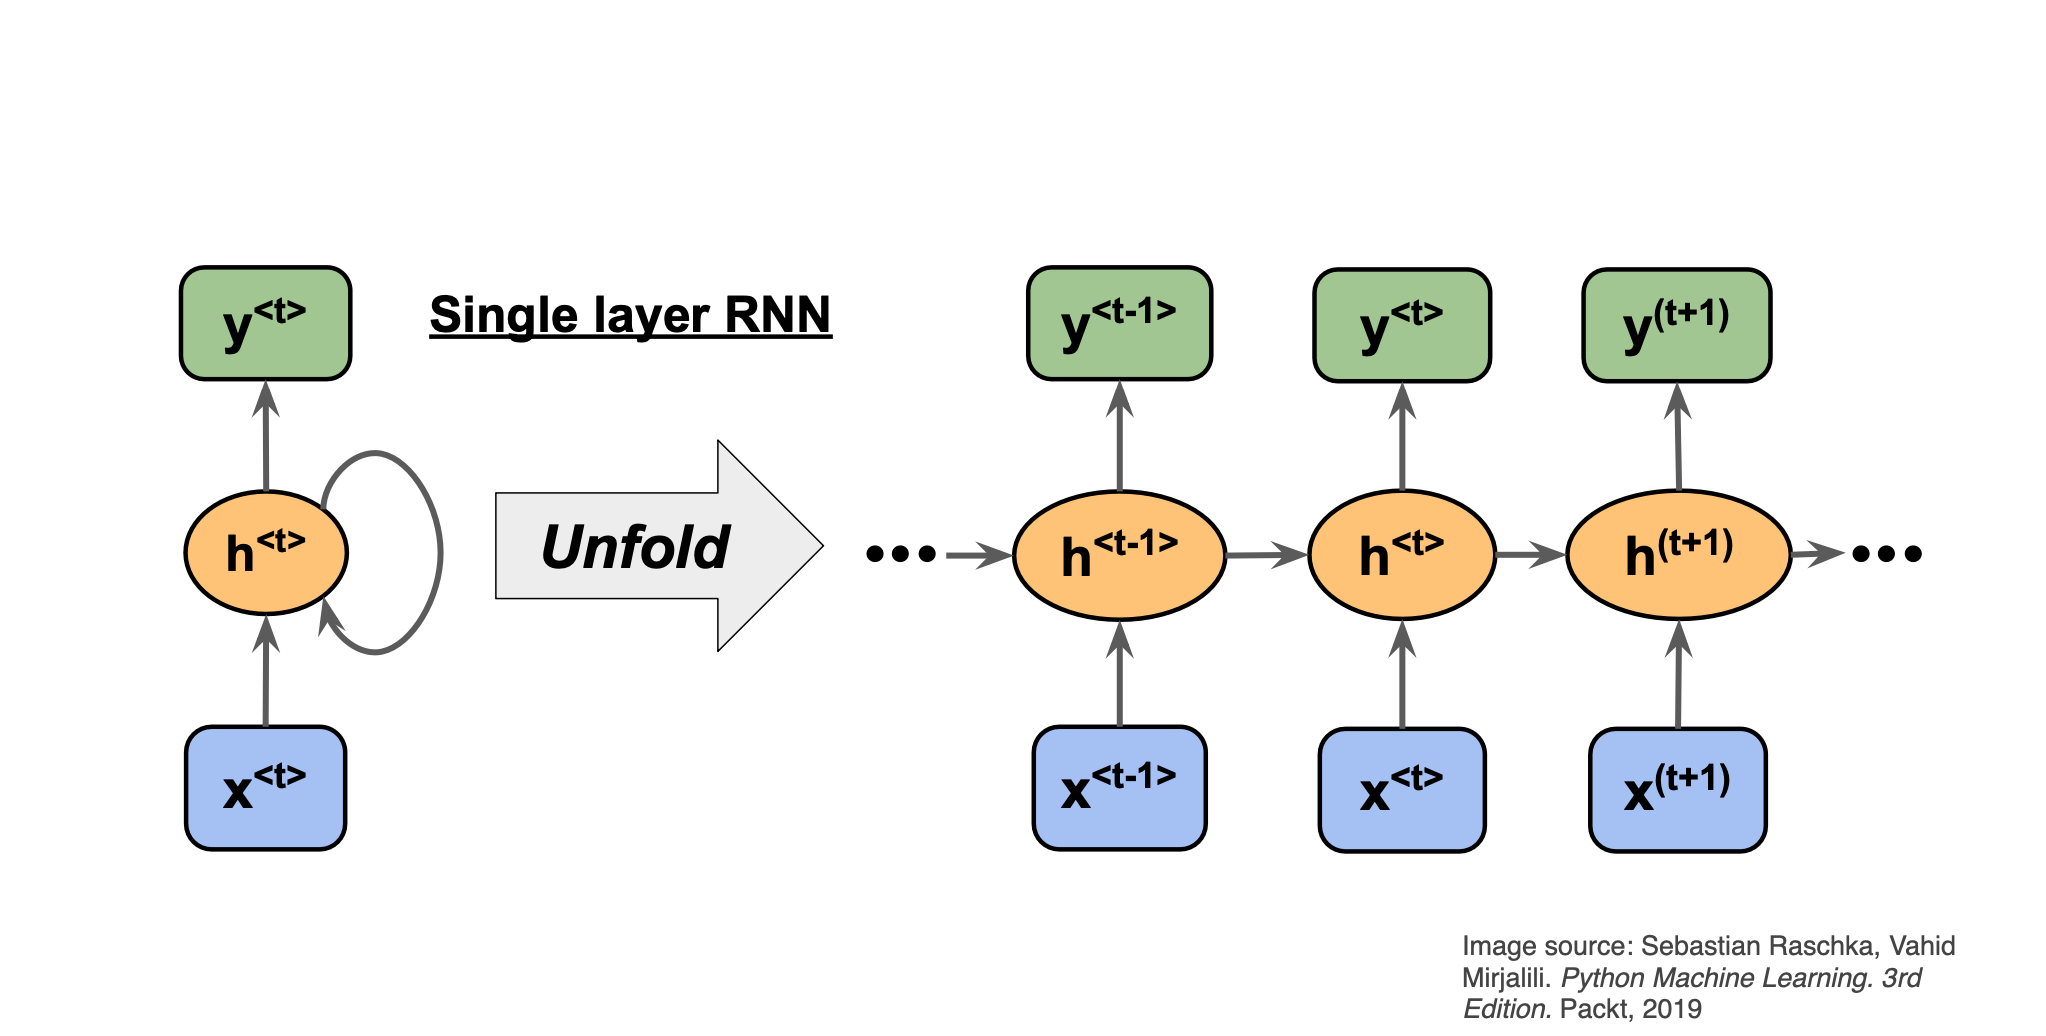
\includegraphics[scale=0.5]{RNN2.png}
 % RNN2.png: 2046x1036 px, 144dpi, 36.09x18.27 cm, bb=0 0 1023 518
 \caption{\textbf{Recurrent Neural Network architecture} Write here}
 \label{fig:RNN}
\end{figure}

\subsubsection{The mathematics of RNNs}
One can have other configurations of an RNN, such as not connecting hidden layers t and t-1, but rather the output of t-1 to the hidden layer of t, and other variants. But sticking with the architecture shown in \autoref{fig:RNN}, the relevant parameters can be seen in \autoref{fig:RNN_w}.

\begin{figure}[!htb]
 \centering
 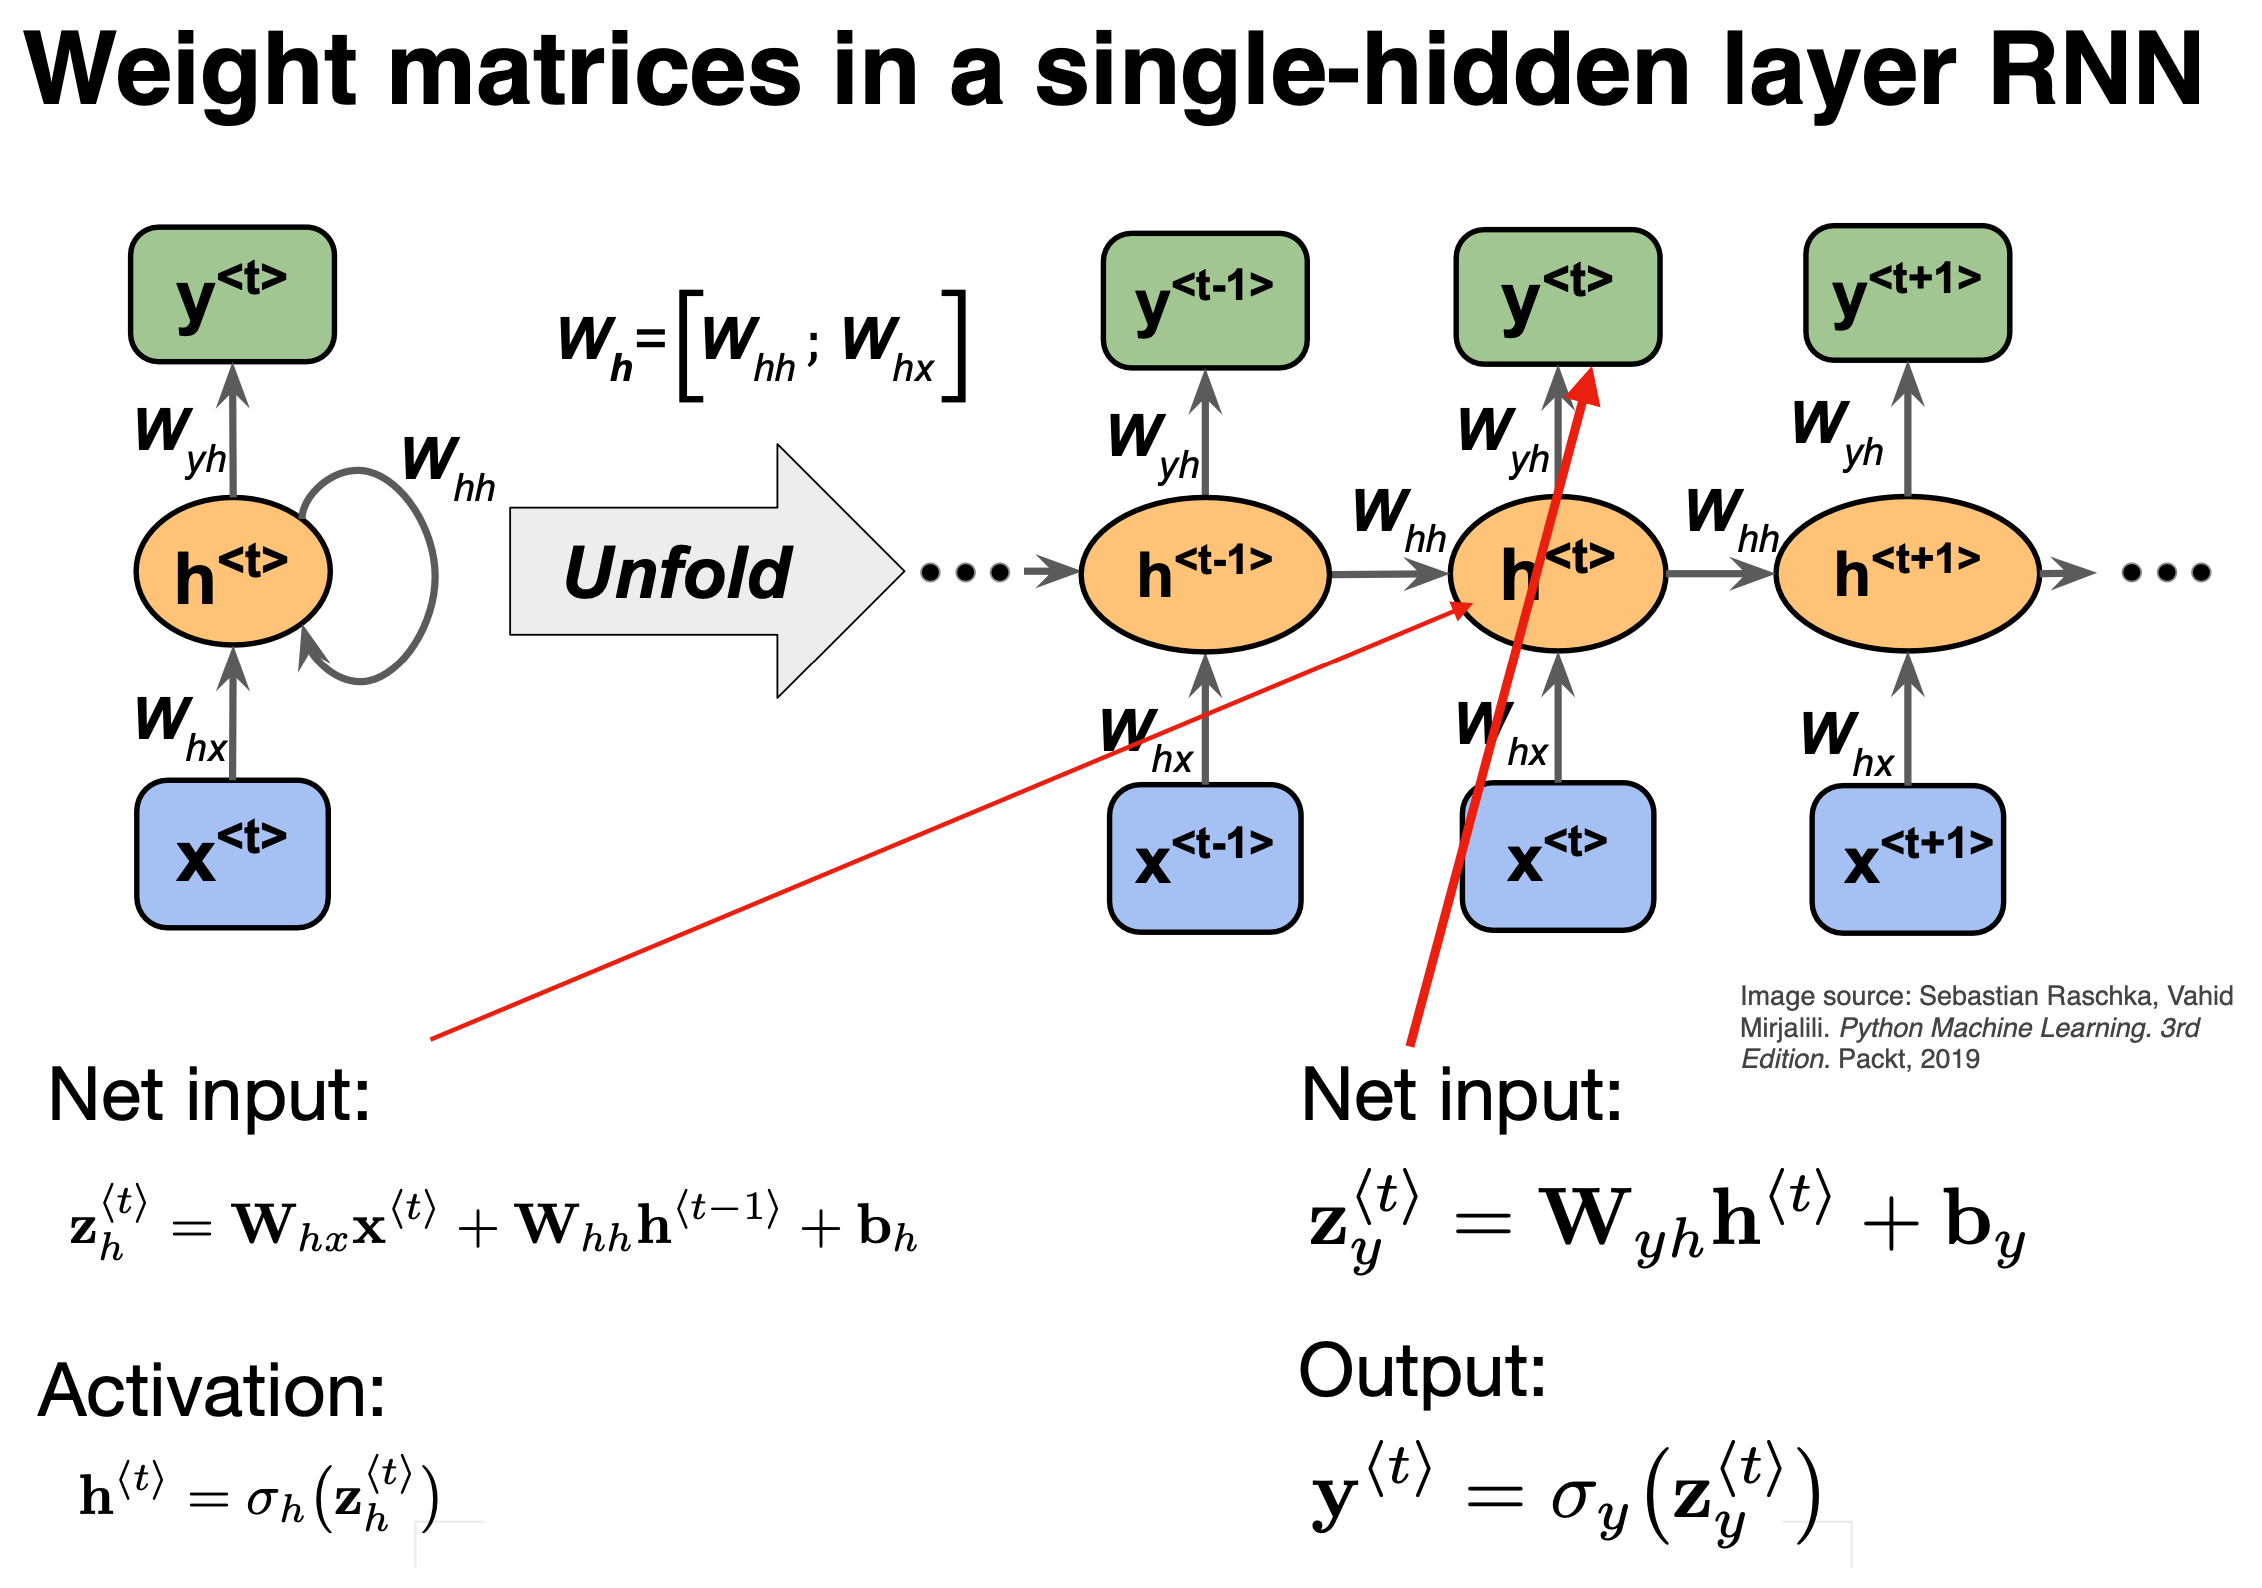
\includegraphics[trim={0cm 0cm 0cm 2.5cm},clip,scale=0.45]{RNN_w.png}
 % RNN_w.png: 2262x1588 px, 144dpi, 39.90x28.01 cm, bb=0 0 1131 794
 \caption{\textbf{RNN parameters}}
 \label{fig:RNN_w}
\end{figure}

Here the inputs to each hidden layer depends on the previous hidden layer as well as the input for this time step, along with the inevitable bias. This input is sent into an activation function such as softmax, and then sent on to the output layer, as well as the next time step hidden layer.
The total loss \textbf{L} can be computed as

\begin{equation}
 L = \sum_{t=1}^TL^{\langle t \rangle},
\end{equation}

where \textbf{L$^{\langle t \rangle}$} is the loss found at time step t. This loss is back propagated through the entire network, so now \textbf{h$^{<t-1>}$} receives 'input' from \textbf{h$^{<t>}$} as well as \textbf{y$^{<t-1>}$}.
The back propagation is done sequentially by the chain rule; wrt to $W_{hh}$

\begin{equation}
 \frac{\partial L}{\partial W_{hh}} = \sum_{t=1}^T\frac{\partial L^{\langle t \rangle}}{\partial W_{hh}} = \sum_{t=1}^T \frac{\partial L^{\langle t \rangle}}{\partial y^{\langle t \rangle}}\frac{\partial y^{\langle t \rangle}}{\partial h^{\langle t \rangle}}\frac{\partial h^{\langle t \rangle}}{\partial W_{hh}}
\end{equation}

The final factor of this equation will depend on the weights $W_{hh}$ and the previous time step hidden layer (which again depends on the previous time step and so on.
Thus we can write (note the lower case t in the summation, summin  only up to the current step):

\begin{equation}
 \frac{\partial h^{\langle t \rangle}}{\partial W_{hh}} = \sum_{k=1}^t \frac{\partial h^{\langle t \rangle}}{\partial h^{\langle k \rangle}} \frac{\partial h^{\langle k \rangle}}{\partial W_{hh}}
\end{equation}

The first factor here can be expanded

\begin{equation}
 \frac{\partial h^{\langle t \rangle}}{\partial h^{\langle k \rangle}} = \frac{\partial h^{\langle t \rangle}}{\partial h^{\langle t-1 \rangle}} \frac{\partial h^{\langle t-1 \rangle}}{\partial h^{\langle t-2 \rangle}}  \cdots \frac{\partial h^{\langle k+1 \rangle}}{\partial h^{\langle k \rangle}} = \prod_{i=k+1}^t \frac{\partial h^{\langle i \rangle}}{\partial h^{\langle i-1 \rangle}}
\end{equation}

If your data consists of many time steps this chain can become extremely long, both increasing computational costs and a long chain can cause exploding gradients as a small change in the initial conditions can lead to large changes in the outcome. 

NICO:
Section on handling exploding gradients? LSTM probably..
Also, total loss should be divided by T (num timesteps) so scale of loss will not be sensitive to length of sequences. not relevant for our purposes I believe, w all sequences as long.

%----------------------------------------------------------------
\subsection{CNN}
%----------------------------------------------------------------
Convolutional Neural Networks (CNNs) are most known for their use in image processing, for tasks such as image recognition, and are characterized by employing convolution in one or more layer instead of matrix multiplications such as in other network types. By assuming a typical image structure on the input data (dimensions of width, height and depth) the architecture of the network can be optimized compared to a more general network. The 3D nature of the input data is kept throughout the hidden layers of the network, which are now subdivided into specific types. In data such as images one would assume some strong (cor)relation between neighboring pixels, which is key to the use of convolution.

First the input is subjected to a convolutional layer, in which a kernel (typically an nxnxf dimension, where we have a filter consisting of f squares of size N$x$N) will scan across the input data, creating an ouput, then translating the kernel sideways by some predefined \textit{stride} length, and repeating the process. In Figure \ref{fig:cnn} an example of the whole CNN process is shown, and in the first step we go from a 28x28x1 size input image, via a 5x5x32 kernel to a 28x28x32 output. When doing a convolution such as this you're no longer interested in a heap of weights and biases as in deep neural nets, but rather just a small set of chosen parameters:

\begin{itemize}
 \item \textbf{Kernel size}: The spatial dimensions of each filter, as well as the number of filters (N$x$N$x$F)
 \item \textbf{Stride}: The distance to move the kernel for each computation. The kernel is moved one stride length to the left each time until it reaches the end of the current row, then it will return to the initial position, move one stride down, and then repeat the whole process.
 \item \textbf{Padding}: Padding refers to adding a rim of zeros (typically) around your image, avoiding potential issues near the edges of the image, as well as to conserve the spatial dimension of the image bein convolved 
\end{itemize}




%inside the window defined by the kernel, computing the output of local regions of the data.
This step will typically increase the depth dimension size considerably, depending on the number of channels in the kernel used.\\



Another important layer type in CNNs is the pooling layer, which decreases the spatial dimensions. In a way it is similar to what we did above, in that we create an N$x$N window again, whisch we apply in a similar manner all over the image. This time however, instead of doing a dot product over the image data and the kernel vaues, we simply find a way of representing the N$x$N data as one single data point. Two very popular methods are to either take the average over all values inside the window, or simply to pick the maximum value.
In Figure \ref{fig:cnn} we see pooling being used in the second operation, where a 2x2 window is applied, quartering the spatial dimension of each channel. Note that this crude dimension reduction can loseinteresting features, so it is rarely chosen to be large.
After a series of such convolutional and pooling layers, you will finally be prepared to do the classification, or whichever task you have for your network. The ouput of your final pooling layer is flattened into a single vector, and sent into one (ore more) fully connected (all to all) layer(s). The output of the final of these is used to perform your designated task.
\begin{figure}[H]
 \centering
 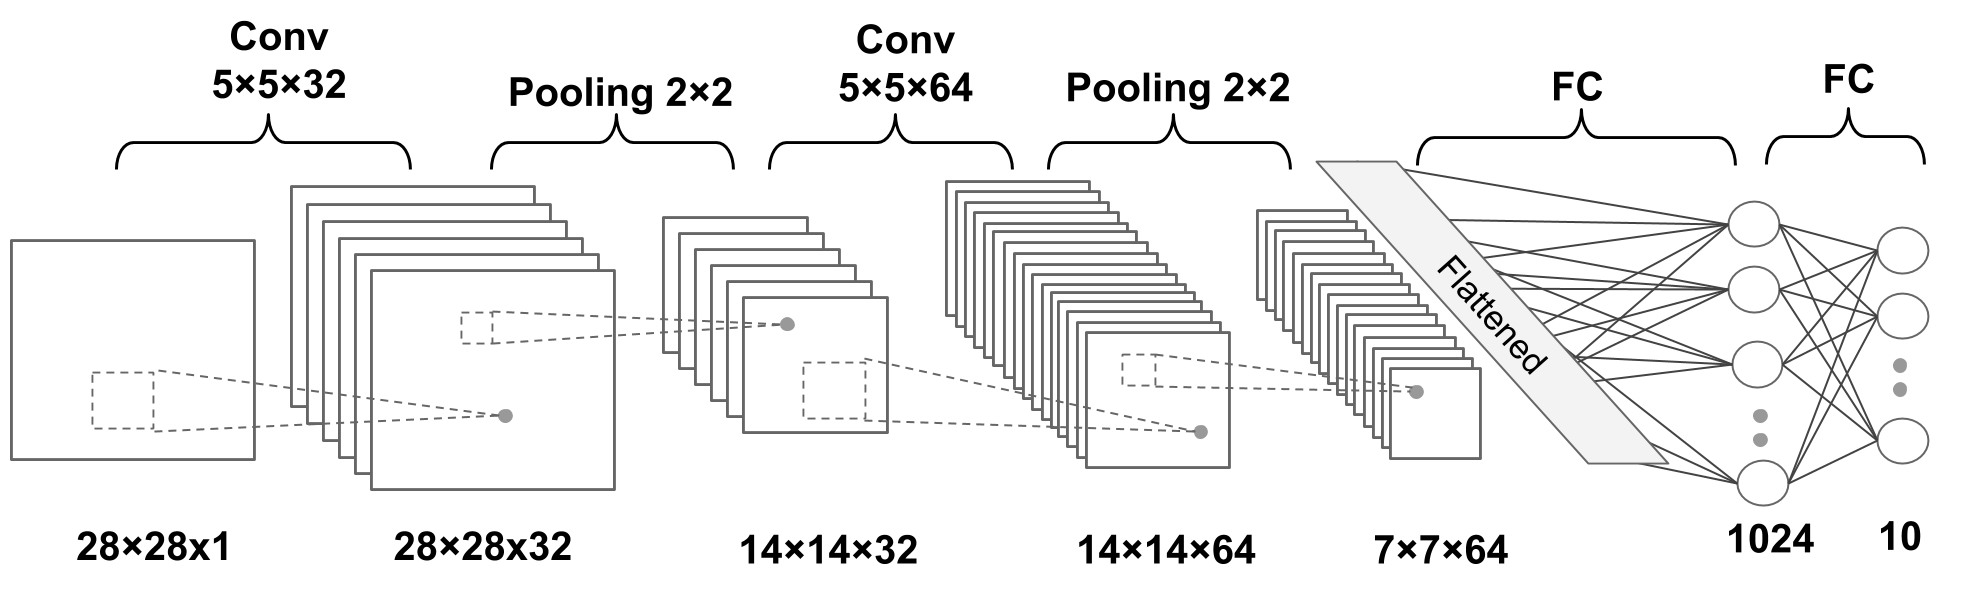
\includegraphics[scale=0.2]{deepcnn.png}
 % deepcnn.png: 1972x595 px, 72dpi, 69.57x20.99 cm, bb=0 0 1972 595
 \caption{\textbf{Convolutional Neural Network architecture} In this figure a simple input, such as a grayscale image, of dimensions 28x28x1 is sent thtough two sets of convolutions and pooling before it is flattened, and sent through a set of fully connected layers (FC) in  the end.}
 \label{fig:cnn}
\end{figure}
Some benefits of such a network compared to a deep neural network are:
\begin{itemize}
 \item they take higher dimensional data as input
 \item not flattening input allows for learning local correlations in all dimensions. Good for feature extraction.
 \item instead of a heap of parameters to chose from, they are very limited per operation
 \item can do unsupervised classification and feature extraction/recognition
\end{itemize}

\subsection{Visualizing the latent space}
It can be useful to find a way to visualize the latent space; such as to see how it is distributed in a 2D space, to see where there may be overlap between features and such.\\
We will be using a method with the fetching name t-distributed stochastic neighbour embedding (t-SNE). In order to represent high dimensional data, such as our latent space visually it makes sense to do a dimensionality reduction down to two (or three) dimensions, as this is easy to draw and comprehend. The method is non-linear and unsupervised, and will emphasize how closely classes (if we're looking at a classification problem, which we usually are when using these embeddings) lie in latent space, and ensure that they lie close in the t-SNE representation. 
This means that t-SNE will calculate a the similarity between all pairs of data points in the data we wish to represent. This can be a rather time-consuming and computationally expensive affair, so datasets containing many (millions) of samples. The similarity is given by a Gaussian distribution,
\begin{equation}
    p_{i|j}=\frac{\exp (-||x_i-x_j||^2/2\sigma_i^2)}{\sum_{k\neq i}\exp(-||x_i-x_k||^2/2\sigma_i^2)},
\end{equation}
the probability that j is a neighbor if you are i. The probabilities will usually be symmetrized, $p_{ij}=(p_{j|i}+p_{i|j})/2N$, where N is the number of samples used.\\ 
A similar probability distribution is created in the low dimensional visualization layer (or embedding space), but here a Student t-distribution is employed in place of the Gaussian distribution we used before: \begin{equation}
    q_{ij}=\frac{(1+||y_i-y_j||^2)^{-1}}{\sum_k\sum_{l\neq k}(1+||y_k-y_l||^2)^{-1}},
\end{equation}
where $q_{ii}=0$.
We now have two probability distributions that we wish to make as similar as possible. But this is something we have recently dealt with, and is done by minimizing the KL divergence!\\
If we call the embedding space distribution Q and the latent space distribution P, we have
\begin{equation}
    D_{KL}(P||Q)=\sum_{i\neq j}p_{ij}\log\frac{p_{ij}}{q_{ij}}
\end{equation}
as the expression we wish to minimize using gradient descent.
Running through these steps should result in a very low (2/3D) representation of a higher dimensional space, that can be used for visualizing classes.\\
